% vim: set ts=4 sw=4
\documentclass[article,a4paper,oneside]{article}
%% Math stuffs
\usepackage[utf8]{inputenc}
\usepackage[english]{babel}
\usepackage[T1]{fontenc}
\usepackage{amssymb}
\usepackage{amsmath}
\usepackage{amsthm}
\usepackage{todonotes}
\usepackage{hyperref}
\usepackage{graphicx}
%%For pseudocode
\usepackage{algorithm2e}
\newtheorem{thm}{Theorem}
\newtheorem{definition}{Definition}
%%We have quite a bit of math inline, so let's remove the paragraph indent and instead move it a bit down
\parindent 0pt
\parskip 4mm
%% for easy Matrix notation
\newcommand{\+}[1]{\ensuremath{\boldsymbol{#1}}}

%%For syntaxhighligting when needed:
%%remember to invoke pdflatex with -shell-escape when not commented out
\usepackage{minted}

\begin{document}
\title{
Randomized Algorithms Project 2\\
A randomized fingerprinting algorithm for efficient computation of multiset equality.
}

\author{
  Mads Ravn - 20071580\\
  Bo Mortensen - 20073241\\
  Johan Abildskov - 20063623
}

\date{\today}

\maketitle

\newpage

\subsection*{Randomized fingerprinting of multisets}
\subsubsection*{Introduction}
In the following report we will describe the results of implementing and testing a fingerprinting algorithm for determining multiset equality based upon $2$-$Universal$ hash functions and \emph{Schwartz-Zippel}.
The issue of determining multiset equality with a deterministic approach is that there are no obvious way that is better than using an efficient sorting algorithm and test for equality. Using the \emph{Schwartz-Zippel} approach also allows us to trivially extend the algorithm to a \emph{streaming} implementation, working efficiently on large datasets. No such approach seems to be possible for the deterministic approach.

\subsection*{Equality of hashed multisets}
\begin{definition}{2-universal hash functions}\\
A hash function h(x) from some universe \emph{U} to a table {T}, where $|U| >> |T|$, is 2\emph{-}universal iff $x \neq y, x,y \in U \Rightarrow Pr[h(x) = h(y)] \leq \frac{1}{|T|}$
\end{definition}
In the rest of the report, $T$ will be $\mathbb{F}_p$ where $p = 2^{31} - 1$, which is a prime.
We now consider two distinct multisets $X = \left[x_1,\cdots, x_n\right]$ and $Y = \left[y_1, \cdots, y_n\right]$. We note that we can assume that both sets have the same size, as it is trivial to determine inequality, if the multisets have different sizes.
We wish to show that using a given hash function $h$, selected uniformly randomly from a family of 2-universal hash functions $H$, $h(X) = \left[h(x_1),\cdots, h(x_n)\right]$ is equal to $h(Y) = \left[h(y_1),\cdots,h(y_n)\right]$ with at most probability $\frac{n}{p}$.
Considering first the element $x_1 \in X$, the probability that $h(x) = h(y)$, for any $y \in Y$ is at most $\frac{n}{p}$ given the 2-universality of $h$ and $|Y| = n$.
An obvious way to improve this bound is to now consider the element $x_2 \in X$ and observe that the probability that this collides with a different $y \in Y$ is $\frac{n-1}{p}$. If these random choices could be shown to be independent we could obtain a better bound from $\prod_{i=0}^{n-1}\frac{n-i}{p}$ which is clearly less than $\frac{n}{p}$. But as this is not the case we will keep the weaker bound $\frac{n}{p}$ which in any case matches the bound obtained from using Schwartz-Zippel later.
\subsection*{Evaluating polynomials of hashed multisets}
We now consider the functions $f_{H(X)}(z) = (z-h(x_1))(z-h(x_2))\ldots(z - h(x_n))$ and $f_{H(Y)}(z) = (z-h(y_1))(z-h(y_2))\ldots(z - h(y_n))$.
We wish to show that if we choose $z$ uniformly at random from $\mathbb{F}_p$ and $f_{H(X)}$ and $f_{H(Y))}$ are distinct polynomials, the probability that we will discover this when evaluating $f_{H(X)}(z)$ and $f_{H(Y)}(z)$ is high. The strategy for showing this is showing that if the two polynomials are indeed distinct, the polynomials will be evaluated to the same value with a probability lower than $\frac{n}{p}$.
To do this we construct a polynomial $g(z) = f_{H(X)}(z) - f_{H(X)}(z)$, it is clear that the two polynomials only evaluate to the same value if $g(z) = 0$. The degree of $g$ is $n$, which comes from the the $n$ $z$ terms in $g$.
As we select $z$ uniformly in $\mathbb{F}_p$, Schwartz-Zippel tells us that $g(z) = 0$ with probability less than $\frac{n}{|\mathbb{F}_p|} = \frac{n}{p}$. As the bound on $g(z)$ gives us a bound on the probability of evaluating distinct polynomials to the same value, we obtain $Pr[f_{H(X)}(z) = f_{H(Y)}(z)] \leq \frac{n}{p}$.

\subsection*{A 2-universal family of hash functions}
As we would like use arithmetic modulo on $p = 2^{31}-1$, we wish to create a family of hash functions that allows us to do work in $\mathbb{F}_p$, even though our elements are of size up to $2^{80}$.

We define $H_s=\{\ h_{a_1,\ldots,a_s}\ | \ a_1,\ldots,a)s\in \mathbb{F}_p\ \}$,
where $h_{a_,\ldots,a_s}(x_1,\ldots,x_s)$.

In order to show that $H_s$ indeed is 2-universal, we have to prove that the probability of a collision $h(x) = h(y)$ is less than $\frac{1}{p}$ if $x \neq y$.

Given two elements $x,y \in U, x \neq y$ and a hash function $h_s \in H_s$, the following holds:
\begin{align*}
h(x) = h(y) &\iff \sum_{i=1}^{s}a_ix_i = \sum_{i=1}^sa_iy_i \\
&\iff \sum_{i=1}^{s}a_ix_i - \sum_{i=1}^sa_iy_i = 0 \\
&\iff a_1x_1 - a_1y_1 + \sum_{i=2}^{s}a_ix_i - \sum_{i=2}^sa_iy_i = 0 \\
&\iff \sum_{i=2}^{s}a_ix_i - \sum_{i=1}^sa_iy_i = a_1(y_i-x_1) \\
&\iff \frac{\sum_{i=2}^{s}a_ix_i - \sum_{i=1}^sa_iy_i}{y_1-x_1} = a_1 \\
\end{align*}
As $x$ and $y$ are given, the only random choices in the above comes from the selection of the variables $a_i$ that fix $h_s \in H_s$. We can now invoke the Principle of deferred decisions and assume that all the other random entries $a_i$ are chosen before $a_1$. This means that the left hand side of the above is fixed at some value $v \in \mathbb{F}_p$. Since $a_1$ is uniformly distributed over $\mathbb{F}_p$ the probability that $a_1 = v$ cannot exceed $\frac{1}{p}$. We have thus shown that $H_s$ as given is a 2 universal function of hash families.
\subsection*{A fingerprinting algorithm}
\begin{algorithm}[multisetfingerprinting]
	\KwData{Multiset}
	\KwResult{Fingerprint in $F_p$}
	$z \gets rand(0..p)$\\
	fix $h_s \in H_s$\\
	$fingerprint \gets 0$\\
	\For{element $e \in input$}{
		$fingerprint \gets fingerprint * (z - h_s(e))$
	}
	\Return{$fingerprint$}

\end{algorithm}
Our proposed algorithm trivially combines the previous sections of this report.
	The above fingerprinting algorithm computes randomized fingerprints of multisets, and uses comparisons of the fingerprints to determine equality.
An input file can be considered as a multiset with each line being an element in the multiset.
The algorithm uses the hash family $H_s$ to hash each element of the multiset. Then we can use the function $f_{H(x)}(z)$ to obtain a fingerprint in $\mathbb{F}_p$ of the multiset.
We can do this for any number of multisets and compare these fingerprints to test for equality.
It is noteworthy that this is a false biased Monte Carlo algorithm, which means that when the algorithm declares two sets distinct, it is always right.
If the two multisets are distinct, based on the previously obtained bound on the probability of evaluating two distinct polynomials to the same value on a uniformly random value $z$, the probability of declaring two distinct sets equal is less than $\frac{n}{p}$.
For an input with $2^{24}$ lines, corresponding to a multiset with $2^{24}$ elements, the probability of a false positive is less than $\frac{2^{24}}{2^{31}-1} \leq 2^{-6}$. To obtain the desired bound on the error probability of $2^{-12}$, we can simply run the algorithm an additional time, if it declares the multisets equal. If we evaluate the polynomials on another independently chosen $z$ we get an error probability of $2^{-6}*2^{-6} = 2^{-12}$.

\subsection*{Implementation}

For our pseudo-random numbers we have used the C++11 Standard Library implementation of the Mersenne Twister number generation algorithm, the std::mersenne\_twister\_engine. Reference: \url{ http://en.cppreference.com/w/cpp/numeric/random/mersenne_twister_engine}. We are using a uniform\_int\_distribution to find a random number in a given range. 

When generating our hash-function, we create a list $a$ of 80 random numbers in the range $[0;p[$ since we know that a line of text can't be longer than 80 characters. When hashing a line we get $h(x) = \sum_{i=0}^{80}a_i*x_i $. Each time we compare two given files/streams we pick a new $z$ to calculate the value of the evaluated pylonomial with. We then compare the value given to each file by this polynomial evaluation. If they are equal we say that the files are equal.

	In our tests we show that we can stream the test-data, but all of our tests are run with the test-data in memory, due to the overhead involved with reading files. The error-prone part of the algorithm has nothing to do with how we read the file, streaming or from memory, so this choice does not alter the results. 

\subsection*{Test results}

We downloaded the 14 multisets from the course site and ran tests on these. We determined that the biggest multisets, data7a and data7b, were pretty big and also equal to eachother, so we didn't run any tets on those. We ran 4 tests on the remaining 6 pairs of multisets and seeing as these were not equal, it gave us some results. First we determined whether two multisets were equal by running the deterministic equality-check: It reads both the files entirely into memory and sort them and then checks element by element if they are equal. After that we ran the randomized equality checks to see whether they gave the same result as the deterministic. When they did not, we counted it as an error.

We noticed that the bigger the multisets are, the more prone to error they are. This is due to us operating within our field of limited space. So the bigger the dataset are, or the smaller the field is, the more likely a hash collision is to happen. An error can also occur when $z-h(x)=0$ because then the rest of the product of the fingerprint function will continue to be $0$. We tried turning down the size of our field in order to see if we would experience more errors - and we did.

\begin{center}
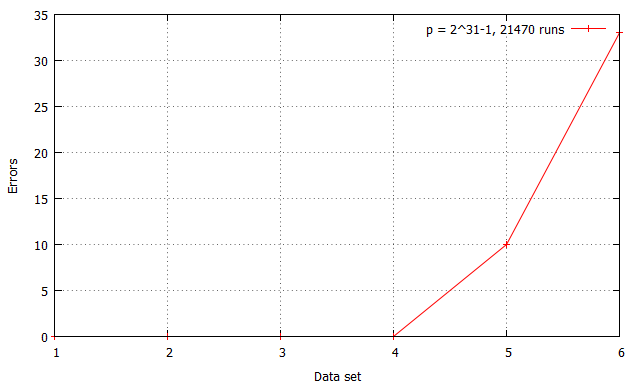
\includegraphics[scale=0.5]{p=2^31-1.png}\\
\end{center}
In this graph we have run our algorithm on the 6 distinct pairs of datasets 104.000 times. As we see, we don't have any errors with datasets of $n\leq 10^4$. In these cases, the error probability is so low that we don't get a single error. With $n=10^4$ our error probability is $\leq \frac{10^4}{2^{31}-1}$, multiplied by the times we ran the algorithm and we should have $\frac{10^4}{2^{31}-1}\cdot 104000 \leq 0,5$ errors and this matches our results nicely.

With $n=10^5$ and $n=10^6$ the expected number of errors are $5$ and $50$, respectively. Our results from dataset 5 exceeds this slightly, but dataset 6 is significantly lower.

\begin{center}
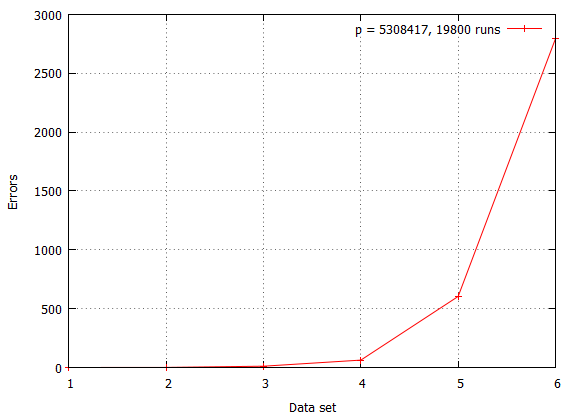
\includegraphics[scale=0.5]{p=5308417.png}\\
\end{center}
In this graph we tried running the algorithm with a decreased $p$. We expected this to give us significantly more errors, and the results proved this we almost a hundred times more errors.

\begin{center}
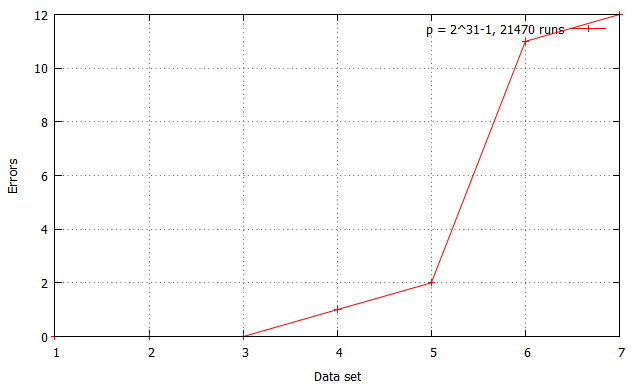
\includegraphics[scale=0.5]{fingerprint_johan.png}\\
\end{center}
In this test we tried changing one of the files in dataset 7 to make them distinct, and although the error probability gives us an expected error amount of $100$, it is only marginally larger than set 6. This could be attributed to the low number of repetitions.

\begin{center}
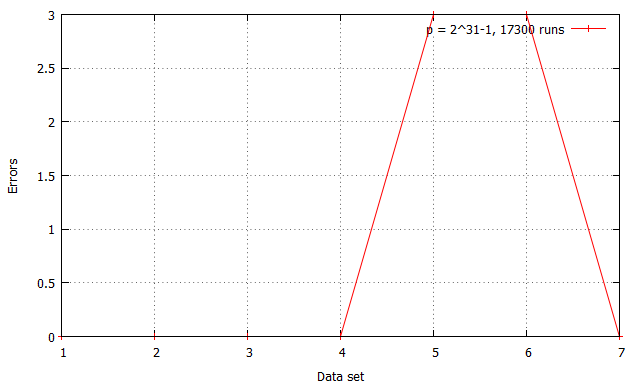
\includegraphics[scale=0.5]{fingerprint_bo.png}\\
\end{center}
Despite being even fewer repetitions this graph shows us, that when dataset 7 is equal, the algorithm always declares them equal.

For the most part of these tests, the results were significantly better than our $\frac{n}{p}$ bound, which suggests that the bound may actually be tighter. The number of results that exceed the bound may get lower with more iterations of the algorithm, but this is uncertain.

If we ran the test twice in each iteration, as the algorithm is described, we would see a decrease in error probability of a factor $\frac{n}{p}$ to get an error probability of $\frac{n^2}{p^2}$, which for datasets of $2^{24}$ elements yields $2^{-12}$.
\subsubsection*{Runtime}
\begin{center}
	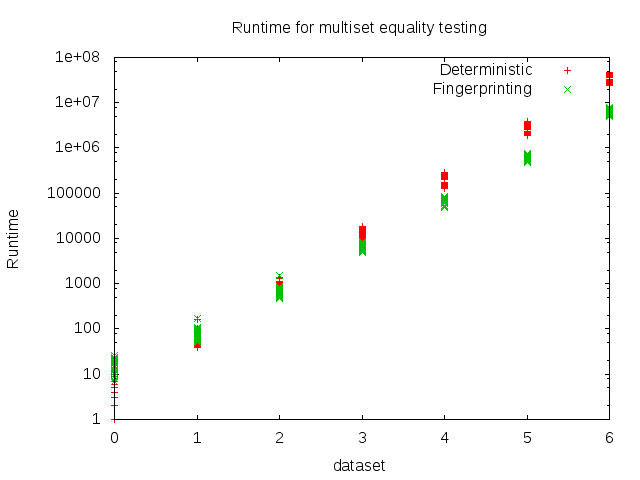
\includegraphics[scale=0.5]{runtime.png}\\
\end{center}
In the graph runtime, we have done a small (3600 iterations) experiment comparing the runtime of the deterministic (sorting) algorithm with that of our fingerprinting algorithm. The runtimes are in nanoseconds and on a logarithmic scale. As can be seen on the graph the randomized algorithm runs quite a bit better than the determistic algorithm as is expected.

\subsection*{Conclusion}
The algorithm that we have designed performs well, both in terms of performance and expected error probability. The algorithm also solves the streaming multiset equality problem using a randomized approach that has no obvious way of being done with a deterministic approach. This is would be particularly useful when using datasets that are too large to fit in main memory, as we use a single sweep through the dataset. A deterministic solution can not do this.

\end{document}
